\documentclass[a4paper,12pt]{report}
\usepackage[utf8]{inputenc}
\usepackage[T1]{fontenc}
\usepackage{times}
\usepackage{mathptmx}
\usepackage[top=1in,left=1.5in,right=1in,bottom=1in]{geometry}
\linespread{1.5}
\usepackage{graphics}
\usepackage{graphicx}
\usepackage{float}
\usepackage{titlesec}
\titleformat{\chapter}
{\Large\bfseries\filcenter}{\thechapter.}{20pt}{\Large}   
\titlespacing*{\chapter}{0pt}{-50pt}{20pt}
\titleformat*{\section}
{\large\bfseries}
\titleformat*{\subsection}
{\normalsize\bfseries}
\titleformat*{\subsubsection}
{\normalsize\bfseries}

\usepackage{pifont}

\usepackage{listings}
\usepackage{color}

\definecolor{dkgreen}{rgb}{0,0.6,0}
\definecolor{gray}{rgb}{0.5,0.5,0.5}
\definecolor{mauve}{rgb}{0.58,0,0.82}

\lstset{frame=tb,
  language=Verilog,
  aboveskip=2mm,
  belowskip=2mm,
  showstringspaces=false,
  columns=flexible,
  basicstyle={\small\ttfamily},
  numbers=none,
  numberstyle=\tiny\color{gray},
  keywordstyle=\color{blue},
  commentstyle=\color{dkgreen},
  stringstyle=\color{mauve},
  breaklines=true,
  breakatwhitespace=true,
  tabsize=3
}

\begin{document}
\pagenumbering{gobble}
\tableofcontents

\newpage
\documentclass[a4paper,12pt]{report}
\usepackage[utf8]{inputenc}
\usepackage[T1]{fontenc}
\usepackage{times}
\usepackage{mathptmx}
\usepackage[top=1in,left=1.5in,right=1in,bottom=1in]{geometry}
\linespread{1.5}
\usepackage{titlesec}
\titleformat{\chapter}[display]
{\normalfont\huge\bfseries\filcenter}{\chaptertitlename\ \thechapter}{20pt}{\Huge}   
\titlespacing*{\chapter}{0pt}{-50pt}{20pt}

\begin{document}
\chapter*{\centering \Large{ABSTRACT}}


\centerline{\emph{\large{\bf A method of Coverage Collection for Stimulus on Emulator }}}
\vspace{10pt}
To verify and to validate a micro-electronic circuit, stimulus is run on varied forms and could come from varied sources. During functional verification of a micro-electronic circuit, coverage is a mechanism to measure effectiveness and completeness of stimulus. On the other hand, we do not have similar mechanisms available for stimulus from other sources where verification simulators cannot be used. It is valuable to generate such coverage information, particularly where it would add value, such as Verification with Emulator. Ever increasing design complexity compels coverage generation and collation over a period of time, say a week or fortnight, as it enables many iteration of stimulus, which is not possible otherwise, due to compute and storage limitations. Such coverage storage and collation tools are already available and is in use in micro-electronic design houses. This project discusses and devises one method of collection, storage and collation of functional coverage for stimulus run on Emulator.



\paragraph{Keywords:}
 \emph{Coverage Database, Emulation, Functional coverage, Simulation, SOC.}

\end{document}


\newpage
\pagenumbering{arabic}
\chapter{INTRODUCTION}

With rapid growth of deep sub-micron technology, there has been an aggressive shrinking in physical dimension of silicon structures that can be realized on silicon. This advancement has enabled the transition of multi million gate designs from large printed circuit boards to SoC (System on Chip). SoC design has the advantages of smaller size, lower power consumption, reliability, performance improvement and low cost per gate. Over the past few years, major challenges faced by semiconductor industry has been to develop more complex SoCs with greater functionality and diversity with reduction in time-to-market. One of the main challenge among this is verification.

Functional verification comprises a large portion of the resources required to design and validate a complex system. Often, the validation must be comprehensive without redundant effort. To minimize wasted effort, coverage is used as a guide for directing verification resources by identifying tested and untested portions of the design. Coverage is defined as the percentage of verification objectives that have been met. It is used as a metric for evaluating the progress of a verification project in order to reduce the number of simulation cycles spent in verifying a design. Coverage collection and management is an important requirement to evaluate the verification progress.

There are two types of coverage metrics: those that can be automatically extracted from the design code, such as code coverage, and those that are user-specified in order to tie the verification environment to the design intent or functionality. The latter form is referred to as functional coverage. Functional coverage is a user-defined metric that measures how much of the design specification, as enumerated by features in the test plan, has been exercised. It can be used to measure whether interesting scenarios, corner cases, specification invariants, or other applicable design conditions, captured as features of the test plan have been observed, validated, and tested. The key aspects of functional coverage are: it is user-specified and is not automatically inferred from the design, it is based on the design specification and is thus independent of the actual design code or its structure.



\section{ORGANIZATION OF THE THESIS}
The organization of this thesis is as follows:\\
\noindent
    {\bf Chapter}~\ref{chap:amd64} gives brief introduction to AMD64 architecture.\\
    {\bf Chapter}~\ref{chap:func_verif} gives brief information on functional verification .\\
    {\bf Chapter}~\ref{chap:coverage} explains about the existing coverage collection methods.\\
    {\bf Chapter}~\ref{chap:coverage_on_emulator} discusses about the proposed enhancements.\\
    {\bf Chapter}~\ref{chap:results} gives final results of the proposed method.\\
    {\bf Chapter}~\ref{chap:conclusion} discusses the various conclusion drawn from the results and the scope for future work.


\newpage
\documentclass[a4paper,12pt]{report}
\usepackage[utf8]{inputenc}
\usepackage[T1]{fontenc}
\usepackage{times}
\usepackage{mathptmx}
\usepackage[top=1in,left=1.5in,right=1in,bottom=1in]{geometry}
\linespread{1.5}
\usepackage{graphics}
\usepackage{graphicx}
\usepackage{float}
\usepackage{titlesec}
\titleformat{\chapter}[display]
{\normalfont\huge\bfseries\filcenter}{\chaptertitlename\ \thechapter}{20pt}{\Huge}   
\titlespacing*{\chapter}{0pt}{-50pt}{20pt}
\titleformat*{\section}{\large\bfseries}

\begin{document}
\chapter*{\centering \Large{AMD64 ARCHITECTURE OVERVIEW}}
\label{chap:amd64}
Typically a SoC brings together functionality that used to be distributed across chips or maybe even devices. Various functional modules of the system are integrated into a single chip set. Naturally SoCs are very complex designs which includes programming elements, hardware elements, software elements, bus architecture, clock and power distribution, test structures etc. 

The heart of any SoC design is a core which is nothing but some sort of processor, and practically all SoC is likely to have at least one processor. In AMD, most processors are based on AMD64 architecture. Majority of the verification scenarios are developed in reference to the behavior of core and hence makes it an important design of interest.

\section {AMD64 ARCHITECTURE}
The AMD64, originally called x86-64, architecture is a 64-bit, backward compatible extension of industry-standard x86 architecture (legacy). It adds 64-bit addressing and expands register resources to support higher performance for recompiled 64-bit programs, while supporting legacy 16-bit and 32-bit applications and operating systems without modification or recompilation. The need for a 64 bit x86 architecture is driven by applications that address large amounts of virtual and physical memory, such as high-performance servers, database management systems, and CAD tools. These applications benefit from both 64-bit addresses and an increased number of registers.



\section {FEATURES OF AMD64}
\addtocontents{toc}{\protect\setcounter{tocdepth}{1}}
The main features of AMD64 architecture are its extended 64-bit registers and new 64-bit mode of operation.  
\subsection{\normalsize{REGISTERS}}

One of the main features of AMD64 architecture is the 64-bit register extension. The small number of registers available in the legacy x86 architecture limits performance in computation-intensive applications. Increasing the number of registers provides a performance boost to many such applications. In addition to the 8 legacy x86 General-Purpose Registers (GPRs), AMD64 introduce additional 8 GPRs. All 16 GPRs are 64-bit long and an instruction prefix (REX) accesses the extended registers. The architecture also introduces 8 new 128-bit media registers.
%\figurename{} 
\begin{figure}[h!]
\centering
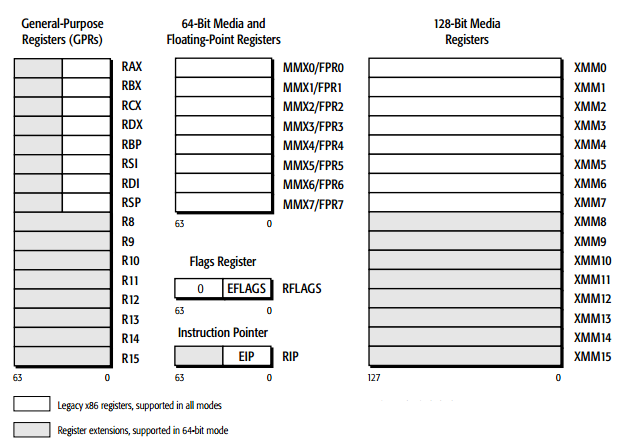
\includegraphics[scale=0.85]{./figures/registers.png}
\caption{AMD64 Registers}
\label{fig:registers.png}
\end{figure}


~\figurename{~\ref{fig:registers.png}} shows the AMD64 application-programming register set. They include the general-purpose registers (GPRs), segment registers, flags register (64-bits), instruction-pointer register (64-bits) and the media registers. 

\subsection{\normalsize{MODES OF OPERATION}}
In addition to the x86 legacy mode, another major feature of AMD64 for is its long mode. This is the mode where a 64-bit application (or operating system) can access 64-bit instructions and registers.%~\figurename{~\ref{fig:modes.eps}} shows the features of each mode of operation in AMD64 architecture. 
The different modes of operations in AMD64 architecture are detailed below:
%\begin{tabular}
%\figurename{} 
%\begin{figure}[h!]

%\centering
%\includegraphics[width=6in]{./figures/modes.eps}
%\caption{AMD64 Modes of Operation}
%\label{fig:modes.eps}
%\end{figure}
%\end{tabular}



\emph {\bf Long Mode}: Long mode is an extension of legacy protected mode. It consists of two sub modes: 64-bit mode and compatibility mode. 64-bit mode supports all of the new features and register extensions of the AMD64 architecture. Compatibility supports binary compatibility with existing 16-bit and 32-bit applications. Long mode does not support legacy real mode or legacy virtual-8086 mode, and it does not support hardware task switching.
\begin{itemize}

\item 64-bit mode: 64-bit mode supports the full range of 64-bit virtual-addressing and register-extension features. This mode is enabled by the operating system on an individual code segment basis. As 64-bit mode supports a 64-bit virtual-address space, it requires a 64-bit operating system and tool chain.


\item Compatibility Mode: Compatibility mode allows 64-bit operating systems to run existing 16-bit and 32-bit x86 applications. These legacy applications run in compatibility mode without recompilation. This mode is also enabled by operating system on an individual code segment bases as in 64 bit mode. However unlike 64-bit mode, x86 segmentation function similar to legacy x86 architecture using 16-bit or 32-bit protected mode semantics.

\end{itemize}



\emph {\bf Legacy Mode}: Legacy mode has compatibility existing 16-bit and 32-bit operating systems in addition to compatibility with existing 16-bit and 32-bit application. Legacy mode has the following three submodes : 

\begin{itemize}

\item Protected Mode: Legacy protected mode supports 16-bit and 32-bit programs with memory segmentation, optional paging, and privilege-checking. Programs in this mode can access up to 4GB of memory space.


\item Virtual-8086 Mode: Virtual-8086 mode supports 16-bit real-mode programs running as tasks under protected mode. It uses a simple form of memory segmentation, optional paging and limited protection-checking. Programs in virtual-8086 mode can access up to 1MB of memory space.


\item Real Mode: Real mode supports 16-bit programs using register-based memory segmentation. It does not support paging or protection-checking. Programs running in real mode can access up to 1MB of memory space.
\end{itemize}

\section{MEMORY ORGANIZATION}
\addtocontents{toc}{\protect\setcounter{tocdepth}{1}}

The AMD64 architecture organizes memory into virtual memory and physical memory. Virtual memory and physical-memory spaces are usually different in size with virtual address space being much larger than physical-address memory.  System software relocates applications and data between physical memory and the system hard disk to make it appear that much more memory is available than what really exist and then uses the hardware memory-management mechanisms to map the larger virtual-address space into the smaller physical-address space.

\subsection {\normalsize{VIRTUAL MEMORY}}
Virtual memory consists of the entire address space available. It is a large linear address space that is translated to a smaller physical address space. Programs uses virtual address space to access locations within the virtual memory space. System software is responsible for managing the relocation of applications and data in virtual memory space using segment-memory management. System software is also responsible for mapping virtual memory to physical memory through the use of page translation.

The architecture supports different virtual-memory sizes using the following modes:
\begin{itemize}

\item[-] Protected Mode: Supports 4 gigabytes of virtual-address space using 32-bit virtual  addresses.

\item[-] Long Mode: Supports 16 exabytes of virtual-address space using 64-bit virtual addresses.
\end{itemize}

\subsection {\normalsize{PHYSICAL MEMORY}}
Physical addresses are used to directly access main memory. This is the installed memory in a particular system that can be physically accessed by the bus interfaces. The larger virtual address space is translated to smaller physical address space through two translation stages called segmentation and paging. The architecture supports different physical-memory sizes using the following modes:
\begin{itemize}

\item[-] Real Mode- Supports 1 Megabyte of physical-address space using 20-bit physical addresses.
\item[-] Legacy Protected Mode- Supports several different address-space sizes, depending on the translation. supports 4 gigabytes of physical address space using 32-bit physical addresses and when the physical-address size extensions are enabled, the page-translation mechanism can be extended to support 52-bit physical addresses.
\item[-] Long Mode- Supports up to 4 petabytes of physical-address space using 52-bit physical addresses. Long mode requires the use of page-translation and the physical-address size extensions (PAE).
\end{itemize}

\section{MEMORY MANAGEMENT}

\addtocontents{toc}{\protect\setcounter{tocdepth}{1}}

Memory management refers to the process involved in translating address generated by software to physical address through segmentation and paging. This process is hidden from application software and is handled by system software and processor hardware. 

\subsection{\normalsize{SEGMENTATION} }
Segmentation mainly helps system software to isolate software processes (tasks) and the data used by that process to increase the reliability of system running multiple process simultaneously. The AMD64 architecture is designed to support all forms of legacy segmentation. In 64-bit mode segmentation is not adopted (use flat band segmentation). Segmentation is, however, used in compatibility mode and legacy mode. 
~\figurename~{\ref{fig:segmentation.png}} shows segmented virtual memory.

%\figurename{} 
\begin{figure}[H]
\centering
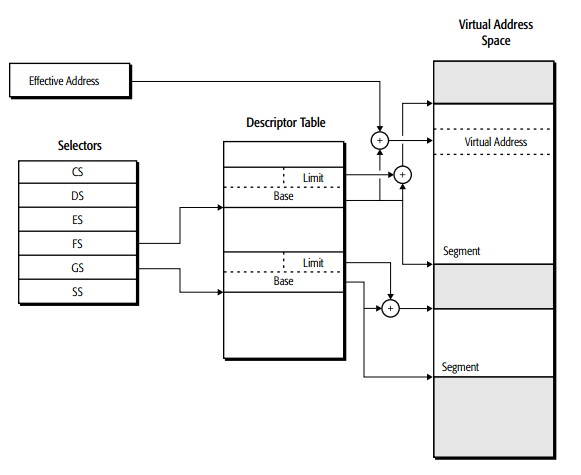
\includegraphics[scale=0.85]{./figures/segmentation.png}
\caption{Segmented Memory Model}
\label{fig:segmentation.png}
\end{figure}


The segmentation mechanism provides ten segment registers, each of which defines a single segment. Six of these registers (CS, DS, ES, FS, GS, and SS) define user segments. The remaining four segment registers (GDT, LDT, IDT, and TR) define system segments. The segment selector points toward a specific entry in descriptor table. This can be Global Descriptor Table (GDT) or Local Descriptor Table (LDT). The descriptor table entry base value plus the effective address which is the offset from base gives the virtual address. Effective address is calculated from the value stored in general purpose register and a displacement value encoded as part of instruction.

\subsection{\normalsize{PAGING}}
Paging allows software and data to be relocated in physical address space using fixed-size blocks called physical pages. It translation uses a hierarchical data structure called a page-translation table to translate virtual pages into physical pages. Paging also provides protection as access to physical pages by lesser-privileged software can be restricted. ~\figurename~{\ref{fig:paging.png}} shows an example of paged memory with three levels in the translation-table hierarchy. 




%\figurename{} 
\begin{figure}[H]
\centering
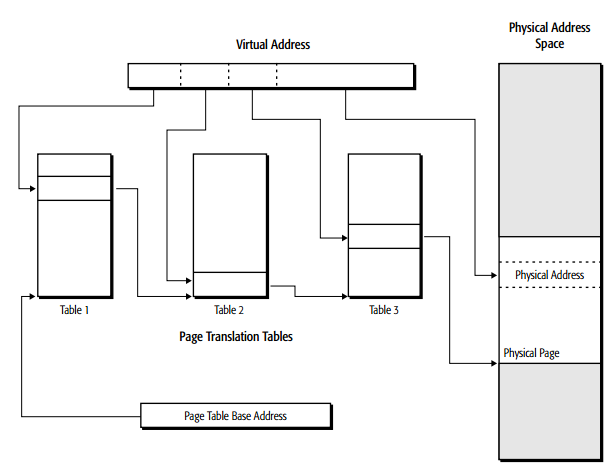
\includegraphics[scale=0.85]{./figures/paging.png}
\caption{Paged Memory Model}
\label{fig:paging.png}
\end{figure}



The number of levels in the translation-table hierarchy can be as few as one or as many as four, depending on the physical-page size and processor operating mode. Each table in the translation hierarchy is indexed by a portion of the virtual-address bits. The entry referenced by the table index contains a pointer to the base address of the next-lower level table in the translation hierarchy. Last page table entry plus the offset value from the virtual address (lsb bits), points toward the actual physical address.  

\end{document}


\newpage
\chapter{FUNCTIONAL VERIFICATION}
\label{chap:func_verif}

\section{INTRODUCTION}
Functional verification involves determining whether or not a logic design matches a specification of its intended behavior. A testbench is built to functionally verify the design by providing meaningful scenarios to check that given certain input, the design performs to specification. In simulation, the testbench wraps around the Design Under Test (DUT), just as a hardware tester connects to a physical chip, as shown in ~\figurename~{\ref{fig:testbench.png}}.
\vspace{10pt}
\begin{figure}[h!]
\centering
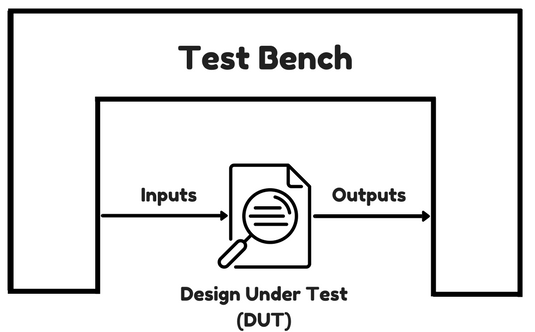
\includegraphics[scale=0.6]{./figures/testbench.png}
\caption{Testbench-Design Environment}
\label{fig:testbench.png}
\end{figure}

\section{LAYERED TESTBENCH}
Layered testbench is a key concept for any modern verification methodology. This kind of testbench makes the task easier by dividing the code into smaller pieces that can be developed separately.
\vspace{10pt}
\begin{figure}[h!]
\centering
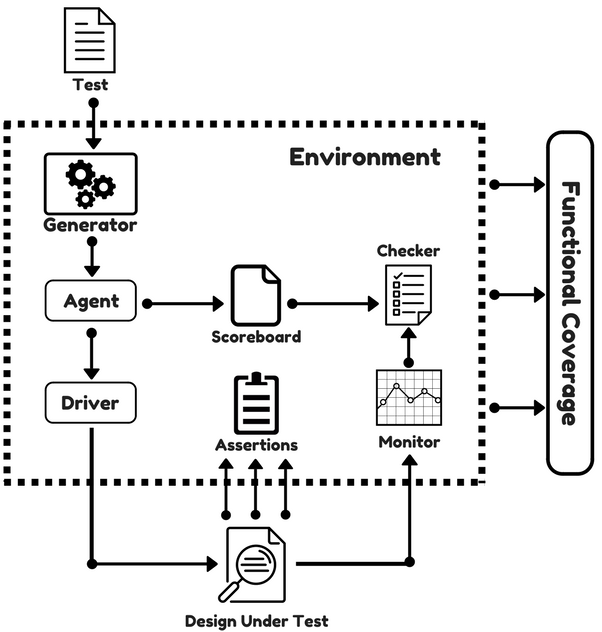
\includegraphics[scale=0.9]{./figures/layered_testbench.png}
\caption{Layered Testbench}
\label{fig:layered_testbench.png}
\end{figure}

\subsection{SIGNAL LAYER}
Signal layer is at the bottom which contains the DUT and the signals that connect it to the testbench.

\subsection{COMMAND LAYER}
The next higher level is the command layer. The DUT’s inputs are driven by the driver that runs single commands, such as bus read or write. The DUT’s output drives the monitor that takes signal transitions and groups them together into commands. Assertions also cross the command/signal layer, as they look at individual signals but look for changes across an entire command.
\paragraph{Driver:} The drivers translate the operations produced by the generator into the actual inputs for the design under verification. Generators create inputs at a high level of abstraction namely, as transactions like read write operation. The drivers convert this input into actual design inputs, as defined in the specification of the designs interface. If the generator generates read operation, then read task is called, in that, the DUT input pin "read-write" is asserted.
\paragraph{Monitor:} Monitor reports the protocol violation and identifies all the transactions. Monitors are two types, Passive and active. Passive monitors do not drive any signals. Active monitors can drive the DUT signals. Sometimes this is also refered as receiver. Monitor converts the state of the design and its outputs to a transaction abstraction level so it can be stored in scoreboard database to be checked later on. Monitor converts the pin level activities in to high level.
\paragraph{Assertions:} Assertions are used to check time based protocols, also known as temporal checks. Assertions are a necessary compliment to transaction based testing as they describe the pin level, cycle by cycle, protocols of the design. Assertions are also used for functional coverage. 

\subsection{FUNCTIONAL LAYER}
Functional layer feeds down into the command layer. The agent block (also called the transactor) receives higher-level transactions such as DMA read or write and breaks them into individual commands. These commands are also sent to the scoreboard that predicts the results of the transaction. The checker compares the commands from the monitor with those
in the scoreboard.
\paragraph{Transactor:} Transactor does the high level operations like burst-operations into individual commands, sub-layer protocol in layered protocol like PciExpress Transaction layer over PciExpress Data Link Layer, TCP/IP over Ethernet etc. It also handles the DUT configuration operations. This layer also provides necessary information to coverage model about the stimulus generated. Stimulus generated in generator is high level like Packet is with good crc, length is 5 and da is 8~Rh0. This high level stimulus is converted into low level data using packing. This low level data is just a array of bits or bytes. Packing is an operation in which the high level stimulus values scalars, strings, array elements and struct are concatenated in the specified manner.
\paragraph{Scoreboard:} Scoreboard is sometimes referred as tracker. Scoreboard stores the expected DUT output. Scoreboard in Verilog tends to be cumbersome, rigid, and may use up much memory due to the lack of dynamic data types and memory allocation. Dynamic data types and Dynamic memory allocation makes it much easier to write a scoreboard in SystemVerilog. The stimulus generator generated the random vectors and is sent to the DUT using drivers. These stimuli are stored in scoreboard until the output comes out of the DUT.
\paragraph{Checker:} The monitor only monitors the interface protocol. It doesn't check the whether the data is same as expected data or not, as interface has nothing to do with the date. Checker converts the low level data to high level data and validated the data. This operation of converting low level data to high level data is called Unpacking which is reverse of packing operation. For example, if data is collected from all the commands of the burst operation and then the data is converted in to raw data , and all the sub fields information are extracted from the data and compared against the expected values. The comparison state is sent to scoreboard. 

\subsection{SCENARIO LAYER}
The generator in the scenario layer drives the functional layer. It generates input vectors that are used to search for anomalies that exist between the intent (specifications) and the implementation.
\paragraph{Generator:} The generator component generates stimulus which are sent to DUT by driver. Stimulus generation is modeled to generate the stimulus based on the specification. For simple memory stimulus generator generates read, write operations, address and data to be stored in the address if its write operation. Scenarios like generate alternate read/write operations are specified in scenario generator. SystemVerilog provided construct to control the random generation distribution and order. Constraints defined in stimulus are combinatioural in nature where as constraints defined in stimulus generators are sequential in nature. 

\subsection{TEST LAYER}
The top-most layer of testbench is the test layer. The test contains the constraints to create the stimulus. Tests can communicate with all the TestBench components.

\subsection{FUNCTIONAL COVERAGE}
Functional coverage measures the progress of all tests in fulfilling the verification plan requirements. The functional coverage code changes through the project as the various criteria complete. This code is constantly being modified, and thus it is not part of the environment.


\newpage
\chapter{COVERAGE COLLECTION AND MANAGEMENT}
\label{chap:coverage}

\section{INTRODUCTION}
Functional coverage management for SOC designs presents a number of requirements not always found at lower levels of the design hierarchy. The coverage model for an SOC is typically a filtered union of all models defined by imported IPs combined with additional coverage terms defined by the SOC team. As such, the number of coverage terms in the SOC model tends to be large in comparison to any individual IP. So, there is an intense need to generate and manage the coverage information. The ~\figurename~{\ref{fig:verif_flow.png}} shows how coverage is generated, merged and stored in a database during the verification.
\vspace{15pt}
\begin{figure}[h!]
\centering
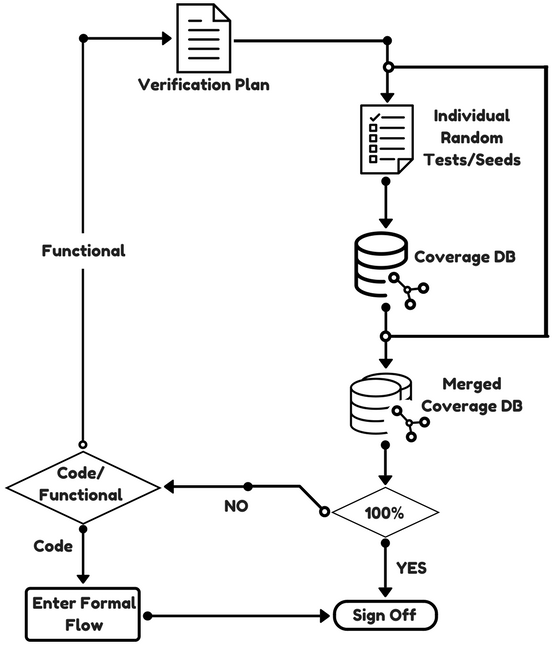
\includegraphics[scale=0.8]{./figures/verif_flow.png}
\caption{Verification Flow}
\label{fig:verif_flow.png}
\end{figure}

\section{COVERAGE COLLECTION FLOW}
After every simulation in a regression, an XML file containing all coverage information for that simulation is generated and copied into a repository unique to that regression. Periodically during the regression, the simulation coverage information residing in the repository is aggregated into a summary coverage XML file. At the end of the regression, only the summary coverage XML file is uploaded. Individual simulation XML coverage results are discarded.
\vspace{15pt}
\begin{figure}[h!]
\centering
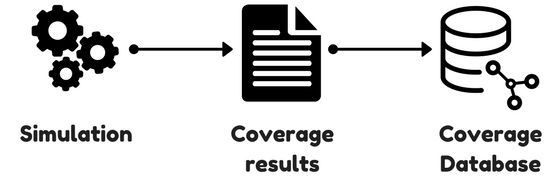
\includegraphics[scale=0.8]{./figures/coverage_collection.png}
\caption{Coverage Collection Flow}
\label{fig:coverage_collection.png}
\end{figure}

\vspace{15pt}
\begin{figure}[h!]
\centering
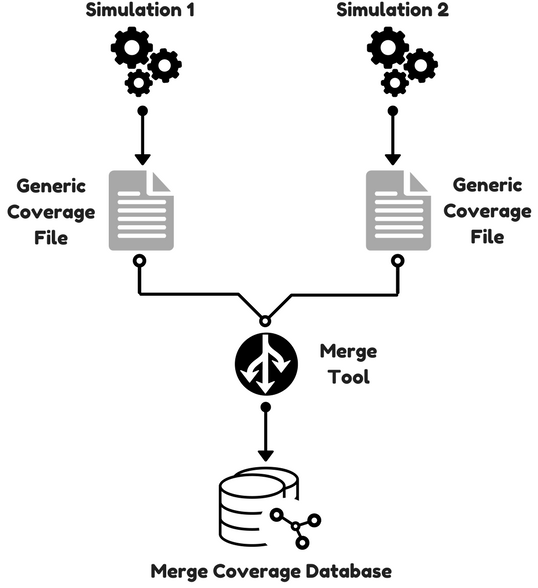
\includegraphics[scale=0.8]{./figures/coverage_management.png}
\caption{Coverage Management Flow}
\label{fig:coverage_management.png}
\end{figure}

\section{EXAMPLE COVERAGE COLLECTION}
Functional coverage model is specified using SystemVerilog. Usually the coverage results are collected by the simulator tools and are dumped in some internal binary format. This example uses \emph{VCS simulator from Synopsys} to illustrate the coverage generation from a testbench. VCS simulation of the testbench generates the coverage and these coverage results are stored in \emph{simv.vdb} directory.

\subsection{TESTBENCH EXAMPLE}
\begin{lstlisting}
module simple_coverage();

logic [7:0]  addr;
logic [7:0]  data;
logic        par;
logic        rw;
logic        en;

covergroup memory @ (posedge en);
  address : coverpoint addr {
    bins low    = {0,50};
    bins med    = {51,150};
    bins high   = {151,255};
  }
  parity : coverpoint  par {
    bins even  = {0};
    bins odd   = {1};
  }
  read_write : coverpoint rw {
    bins  read  = {0};
    bins  write = {1};
  }
endgroup

memory mem = new();

task drive (input [7:0] a, input [7:0] d, input r);
  #5 en <= 1;
  addr  <= a;
  rw    <= r;
  data  <= d;
  par   <= ^d;
  $display ("@%2tns Address :%d data %x, rw %x, parity %x",$time,a,d,r, ^d);
  #5 en <= 0;
  rw    <= 0;
  data  <= 0;
  par   <= 0;
  addr  <= 0;
  rw    <= 0;
endtask

initial begin
  en = 0;
  repeat (10) begin
    drive ($random,$random,$random);
  end
  #10 $finish;
end

endmodule

\end{lstlisting}

\subsection{SIMULATION OUTPUT}
\begin{verbatim}
@ 5ns Address : 36 data 81, rw 1, parity 0
@15ns Address : 99 data 0d, rw 1, parity 1
@25ns Address :101 data 12, rw 1, parity 0
@35ns Address : 13 data 76, rw 1, parity 1
@45ns Address :237 data 8c, rw 1, parity 1
@55ns Address :198 data c5, rw 0, parity 0
@65ns Address :229 data 77, rw 0, parity 0
@75ns Address :143 data f2, rw 0, parity 1
@85ns Address :232 data c5, rw 0, parity 0
@95ns Address :189 data 2d, rw 1, parity 0
\end{verbatim} 

\subsection{COVERAGE REPORT}
Simulation of the testbench using VCS simulator generates \emph{simv.vdb} which is the \emph{Verification Database directory}. VCS writes intermediate files and reports about coverage in the form of XML files in subdirectories within in this directory.

To view the coverage report, a reporter utility of VCS named \emph{'urg'} is used.
\vspace{15pt}
\begin{figure}[h!]
\centering
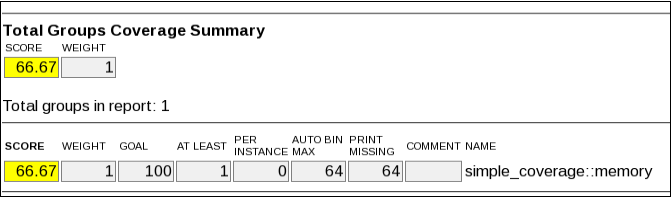
\includegraphics[scale=0.85]{./figures/urgreport2.png}
%\caption{}
\label{fig:urgreport2.png}
\end{figure}

\begin{figure}[h!]
\centering
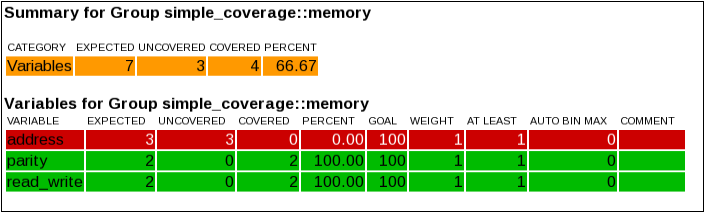
\includegraphics[scale=0.85]{./figures/urgreport3.png}
%\caption{}
\label{fig:urgreport3.png}
\end{figure}

\begin{figure}[h!]
\centering
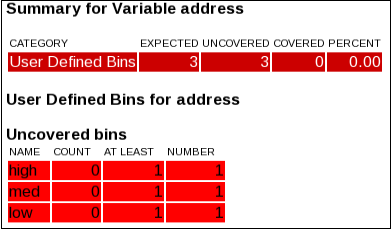
\includegraphics{./figures/urgreport4.png}
%\caption{}
\label{fig:urgreport4.png}
\end{figure}

\begin{figure}[h!]
\centering
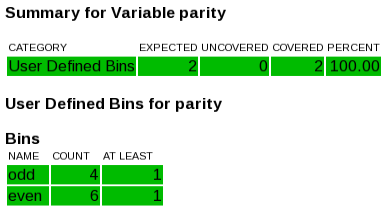
\includegraphics{./figures/urgreport5.png}
%\caption{}
\label{fig:urgreport5.png}
\end{figure}

\begin{figure}[h!]
\centering
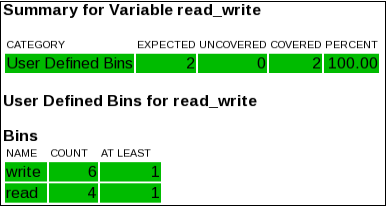
\includegraphics{./figures/urgreport6.png}
%\caption{}
\label{fig:urgreport6.png}
\end{figure}


\newpage
\chapter{COVERAGE COLLECTION ON EMULATOR}
\label{chap:coverage_on_emulator}

\section{INTRODUCTION}
As the design complexity is increasing over time, it is important to generate and collate coverage. Coverage information is generated when verification of a design is done with a Simulator. Whereas, when there is a need to verify using an Emulator, coverage information is not generated. This chapter discusses a method for coverage collection on Emulator.
\section{EMULATION}
An emulation is the process of imitating the behavior of one or more pieces of hardware (typically a system under design) with another piece of hardware. It is like duplicating every aspect of the original device’s behaviour. It is effectively a complete replication of another system, right down to being binary compatible with the emulated system's inputs and outputs, but operating in a different environment to the environment of the original emulated system. The rules are fixed, and cannot be changed or the system fails.

The advantage of emulation is that it combines the programming flexibilities of simulators with the performance and system integration advantages of a hardware model. It allows testing of ASIC designs in a full system environment operating at reduced frequencies. This offers the opportunity to debug the design more thoroughly prior to release to silicon and to start software development on the complete system much earlier in the development cycle.

\section{EMULATION VS. SIMULATION}
\begin{itemize}

\item[\ding{51}] Simulation is a serial software algorithm computing circuit behavior with vectors or other stimulus.

\item[\ding{51}] Emulation is actual hardware performing simultaneous tasks using vectors or real target systems for stimulus.
  \begin{itemize}
    
  \item It is upto 100,000 times faster than Simulation.

  \item It verifies functionality in target system environment.
  \item Emulation finds functional system problems before silicon.
  \item It allows concurrent development and debugging of hardware, software and systems.
    \end{itemize}
  
\end{itemize}

\section{EMULATION MODES}
Emulation modes are characterized by the type of stimulus applied to DUT.
\subsection{SIGNAL BASED ACCELERATION}
In this mode, an RTL testbench drives the DUT in the emulator via a programmable logic interface (PLI). In general, this is the slowest performance mode, but it has some advantages, such as the fact that it does not require changes to the testbench. It is just 5-50 times faster and runs with PLI compliant simulator or native c++.
\subsection{TRANSACTION BASED ACCELERATION}
Transaction-based emulation mode moves verification to an upper  level of abstraction from the register transfer level (RTL), improving performance and debug productivity. It is 50-500 times faster and transactional testbench is required and tuned for efficiency.
\subsection{EMBEDDED TESTBENCH ACCELERATION}
In this mode, the software code is executed on the DUT processor mapped inside the emulator. This is the fastest performance mode, making it the choice for processing billions of verification cycles necessary to boot an operating system. This is 1000-100,000 times faster and needs synthesizable testbench.
\subsection{IN CIRCUIT EMULATION}
This was considered to be the traditional method when hardware emulation was deployed. In this case, the DUT is mapped inside the emulator and connected in in-circuit emulation (ICE) mode to the target system in place of a chip or processor for debug prior to silicon availability.

\section{EMULATOR TYPES}
An Emulator is a system of hardware and software to test actual target systems. Following are Emulator types from different vendors:
\begin{itemize}

\item Palladium (Cadence)
\item Xtreme (Cadence/Axis)
\item Veloce (Mentor Graphics)
\item ZeBu (EVE)
  
\end{itemize}

\section{PROPOSED COVERAGE COLLECTION FLOW}
Once the Emulation runs are performed on tests, a transaction log file is generated. The required information for which the coverage is to be generated is extracted from the log file using c/c++ and a testbench is written for coverage using SystemVerilog. Verilog PLI is used to interface SystemVerilog simulations to c/c++ models. This combined code is then simulated using VCS simulator which generates simv.vdb directory from which the coverage information is uploaded to a coverage database wherein the the filtering, merging and waivering of the coverage is performed by the coverage tool.
\vspace{15pt}
\begin{figure}[h!]
\centering
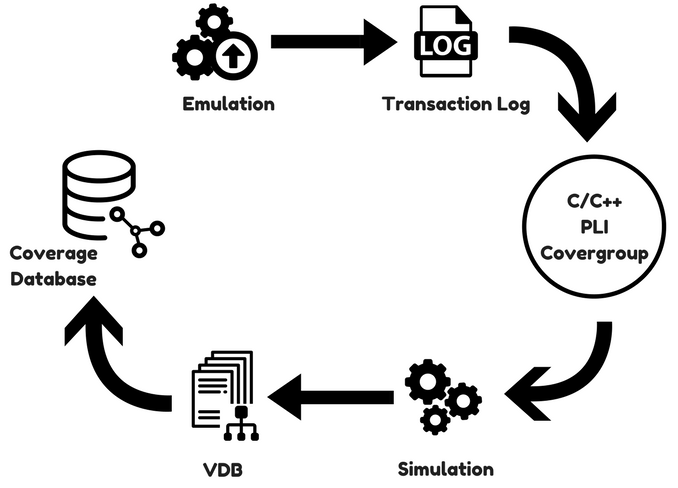
\includegraphics[scale=0.8]{./figures/coverage_collection_on_emulator.png}
\caption{Coverage collection on emulator}
\label{fig:coverage_collection_on_emulator.png}
\end{figure}

\section{C++ Language}
C++ is a general purpose programming language. It has imperative, object-oriented and generic programming features, while also providing facilities for low-level memory manipulation.
\section{VERILOG PLI}
The Verilog Programming Language Interface (Verilog PLI), is one of the more powerful features of Verilog. The PLI provides a means for both hardware designers and software engineers to interface their own programs to commercial Verilog simulators. Through this interface, a Verilog simulator can be customized to perform virtually any engineering task desired. Few common uses of the PLI include interfacing Verilog simulations to C language models, adding custom graphical tools to a simulator, reading and writing proprietary file formats from within a simulation, performing test coverage analysis during simulation etc.
\section{FUNCTIONAL COVERAGE}
Functional coverage is a user-defined metric in SystemVerilog that measures how much of the design specification, as enumerated by features in the test plan, has been exercised.\\
The key aspects of functional coverage are as follows:
\begin{itemize}
\item[-] It is user-specified and is not automatically inferred from the design.
\item[-] It is based on the design specification and is thus independent of the actual design
code or its structure.
\end{itemize}
\subsection{COVERGROUP}
The covergroup construct encapsulates the specification of a coverage model. Each covergroup specification can include the following components:
\begin{itemize}
\item[-] A clocking event that synchronizes the sampling of coverage points
\item[-] A set of coverage points
\item[-] Cross coverage between coverage points
\item[-] Optional formal arguments
\item[-] Coverage options
\end{itemize}
\subsubsection{Coverpoint}
A covergroup can contain one or more coverage points. A coverage point specifies an integral expression that is to be covered. Each coverage point includes a set of bins associated with the sampled values or value transitions of the covered expression. The bins can be explicitly defined by the user or automatically created by SystemVerilog.


\newpage
\chapter{IMPLEMENTATION RESULTS}
\label{chap:results}
\vspace{15pt}
\begin{figure}[h!]
\centering
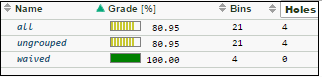
\includegraphics{./figures/coverage_db.png}
\caption{}
\label{fig:coverage_db.png}
\end{figure}

\vspace{15pt}
\begin{figure}[h!]
\centering
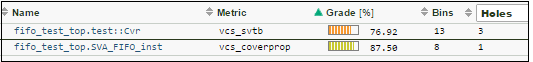
\includegraphics{./figures/coverage_db1.png}
\caption{}
\label{fig:coverage_db1.png}
\end{figure}

\vspace{15pt}
\begin{figure}[h!]
\centering
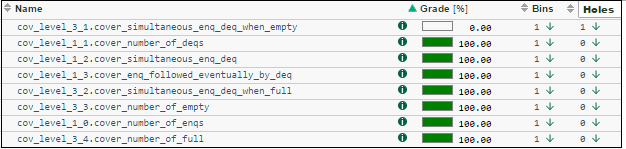
\includegraphics{./figures/coverage_db2.png}
\caption{}
\label{fig:coverage_db2.png}
\end{figure}


\newpage
\chapter{CONCLUSION}
\label{chap:conclusion}


\end{document}

